\documentclass[a4paper,12pt,oneside]{report}

\usepackage[utf8]{inputenc}
\usepackage[T1]{fontenc}
\usepackage{geometry}
\usepackage{setspace}
\usepackage{graphicx}
\usepackage{float}
\usepackage{array}
\usepackage{booktabs}
\usepackage{tabularx}
\usepackage{xcolor}
\usepackage{tikz}
\usetikzlibrary{arrows.meta,positioning,shapes.geometric,fit,calc}
\usepackage{adjustbox}
\usepackage{microtype}
\usepackage{xurl}
\usepackage[nottoc]{tocbibind}
\usepackage{hyperref}

% Binding margin: extra space on the left so text is not hidden after hard-binding.
% Top, bottom and right stay equal.
\geometry{left=1.5in, right=1.0in, top=1.0in, bottom=1.0in}
\setstretch{1.15}
\emergencystretch=3em
\graphicspath{{screenshots/}{figures/}}
\hypersetup{colorlinks=true,linkcolor=black,citecolor=black,urlcolor=blue}
\urlstyle{same}

\newcolumntype{Y}{>{\centering\arraybackslash}X}
\newcolumntype{L}{>{\raggedright\arraybackslash}X}
\newcommand{\code}[1]{\path{#1}}

\newcommand{\projtitle}{GestureTalk: Real-Time Sign Language Recognition, Text Conversion and Speech Generation System}

\begin{document}

% ===================== TITLE PAGE =====================
\begin{titlepage}
    \centering
    \vspace*{0.5cm}

    {\Large \textbf{\projtitle}\par}
    \vspace{0.5cm}
    {\large Project Report\par}
    \vspace{0.8cm}

    A report submitted for the course\par
    \vspace{0.25cm}
    {\large \textbf{CS4203 -- Project-II / Internship}\par}

    \vspace{0.6cm}
    {\large SEMESTER -- VII\par}
    \vspace{0.6cm}

    \IfFileExists{screenshots/iiit-manipur.png}{%
        
\includegraphics[width=3.6cm]{screenshots/iiit-manipur.png}%
    }{%
        {\large\textit{Indian Institute of Information Technology Senapati, Manipur}}%
    }
    \vspace{0.9cm}

    Submitted By\par
    \vspace{0.2cm}
    {\Large \textbf{MOHIT GORA}}\\
    SEMESTER -- VII\\
    Roll No: \textbf{230101056}

    \vspace{0.7cm}
    Supervised By\par
    \vspace{0.2cm}
    {\Large \textbf{Dr. Sanasam Chanu Inunganbi}}

    \vfill
    {\large Department Of Computer Science And Engineering\\
    Indian Institute of Information Technology Senapati, Manipur\\
    Submission Date: \underline{\hspace{3cm}}}
\end{titlepage}

% ===================== DECLARATION =====================
\chapter*{Declaration}
In this submission, I have expressed my idea in my own words, and I have adequately cited and referenced any ideas or words that were taken from another source. I also declare that I adhere to all principles of academic honesty and integrity and that I have not misrepresented or falsified any ideas, data, facts, or sources in this submission. If any violation of the above is made, I understand that the institute may take disciplinary action. Such a violation may also engender disciplinary action from the sources which were not properly cited or permission not taken when needed.

\vspace{1.4cm}
\hfill
\begin{tabular}{@{}l@{}}
MOHIT GORA \\[0.45cm]
230101056 \\[0.45cm]
DATE: \underline{\hspace{3.2cm}}
\end{tabular}

\newpage

% ===================== CERTIFICATE =====================
\thispagestyle{empty}
\begin{center}
\IfFileExists{screenshots/iiit-manipur.png}{
\includegraphics[scale=0.16]{screenshots/iiit-manipur.png}\\[0.25cm]}{}
\begin{tabular}{l}
Department of Computer Science and Engineering \\
Indian Institute of Information Technology Senapati, Manipur \\
\end{tabular}
\end{center}
\par\noindent\rule{\textwidth}{0.4pt}
Dr.\ Sanasam Chanu Inunganbi
\hfill Email: \href{mailto:inunganbi@iiitmanipur.ac.in}{inunganbi@iiitmanipur.ac.in}\\
Assistant Professor\\[1.1cm]
{\LARGE \textbf{\emph{To Whom It May Concern}}}\\[1.0cm]
This is to certify that the project report entitled \textbf{``GestureTalk: Real-Time Sign Language Recognition, Text Conversion and Speech Generation System''}, submitted to the Department of Computer Science and Engineering, Indian Institute of Information Technology Senapati, Manipur, in partial fulfillment of the requirements for the award of the degree of Bachelor of Technology in Computer Science and Engineering, is a record of bona fide work carried out by \textbf{MOHIT GORA} bearing roll number \textbf{230101056} for the course \textbf{CS4203 -- Project-II / Internship}.\\[1.1cm]
\hfill Signature of Supervisor\\[0.15cm]
\hfill \textbf{Dr.\ Sanasam Chanu Inunganbi}\\[0.7cm]
Signature of Examiner 1 \dotfill\\[0.3cm]
Signature of Examiner 2 \dotfill\\[0.3cm]
Signature of Examiner 3 \dotfill\\[0.3cm]
Signature of Examiner 4 \dotfill

\newpage

% ===================== ABSTRACT =====================
\chapter*{Abstract}
GestureTalk is a real-time desktop system that watches one hand through a laptop webcam, converts the pose into an English word on the screen, and speaks the same word through the computer speakers. The work grew from a simple observation. In classrooms, offices and public counters, speech is treated as the default way to communicate. A person who relies on hand signs then depends on someone nearby who already understands those signs. A small local program cannot replace a full natural sign language, but it can give an immediate word and a spoken sentence when a known pose is held in front of the camera.

The present implementation runs entirely on a Windows laptop. OpenCV captures a mirrored live frame. MediaPipe Tasks HandLandmarker returns twenty-one normalised landmarks. A project-specific classifier then reads finger extension, pointing direction and left or right hand, and maps the pose onto a custom vocabulary of more than five hundred everyday gestures. The recognised label is not accepted on the first noisy frame. Separate open and close thresholds, a short majority window and a hold of about one tenth of a second keep the overlay steady. Speech is generated offline by the Windows speech engine in a background thread, so a new pose can interrupt the previous utterance without freezing the camera loop.

The system is a working college prototype, not a complete American or Indian Sign Language interpreter. It is meant for a live demonstration of tracking, recognition, text conversion and speech generation, and for later replacement of the rule table by a trained model. The contribution of this stage is an original, offline path from webcam to spoken word, with a large everyday vocabulary that can be shown in a viva.

\newpage

% ===================== ACKNOWLEDGEMENT =====================
\chapter*{Acknowledgement}
I express my sincere gratitude to \textbf{Dr.\ Sanasam Chanu Inunganbi} for guidance during this project. The regular discussions helped me keep the design honest: what the camera can really see, what the classifier can really decide, and what should be left for later work. I am also thankful to the Department of Computer Science and Engineering, Indian Institute of Information Technology Senapati, Manipur, for the opportunity to carry out CS4203 Project-II in this area.

\tableofcontents
\listoffigures
\listoftables
\newpage

\chapter{Introduction}
\section{Overview}
GestureTalk is a local Python application that turns a live hand pose into on-screen English text and then into speech. The user sits in front of a webcam, shows one hand, holds a pose for a short moment, and sees a word such as HELLO, HELP or WATER on the OpenCV window. The same word is spoken by the Windows speech engine without sending audio to a cloud service. Tracking uses the current MediaPipe Tasks HandLandmarker rather than the older Hands module that many public samples still call. Classification at this stage is landmark geometry. A trained image network is planned, but it is not claimed as part of the running demo.

The vocabulary built for the project contains more than five hundred gestures. Everyday words covering greetings, family, school, food, travel, numbers, colours and common actions were added so that a short viva can show several useful poses instead of a handful of letters. Named shapes such as HELLO, I LOVE YOU, YES, NO, PEACE and OK sit on top of that table and are recognised from well known finger patterns.

\section{Background and Motivation}
Spoken language is the default channel in most public spaces. A person who cannot speak, or who is more comfortable with signed communication, is often left waiting for a human interpreter. Public sign-recognition samples exist, but many of them stop at the alphabet, depend on an outdated MediaPipe API, change the label on every frame, or send text to a paid online speech service. Those limits make the samples hard to run in a classroom viva and hard to defend as original student work.

A practical college prototype therefore needs to run on an ordinary laptop, produce a word that can be shown and spoken in real time, stay offline, and remain simple enough to explain. GestureTalk is motivated by that accessibility gap and by those engineering constraints. It does not attempt to model the grammar or facial markers of a natural sign language. It tries to close a smaller loop: one hand, one stable word, one spoken sentence.

\section{Problem Statement}
Given a live webcam image of a single hand, the system must produce a stable English label and speak that label locally. The label should not flicker every time a fingertip crosses a threshold. Speech should not block the camera thread. The implementation should use a current hand-tracking API and original application code. The problem is therefore not ``solve sign language'' in the linguistic sense. The problem is to build a complete, honest, real-time path from camera to text and speech, with a large enough vocabulary that the demonstration is useful.

\section{Objectives}
The first objective is to capture a webcam frame, mirror it for a natural selfie view, and extract twenty-one hand landmarks. The second is to classify a custom vocabulary of more than five hundred gestures from finger extension, hand orientation and corrected handedness. The third is to keep the overlay stable using per-finger hysteresis, a short majority window and hold-to-confirm. The fourth is to speak each newly confirmed gesture once, offline, without waiting for audio to finish. The fifth is to keep the code modular so that a trained model can replace the rule table in a later stage without rewriting the camera loop.

\section{Scope}
The current scope is a single-user Windows application with one webcam and one hand. It covers tracking, custom pose classification, smoothing, on-screen text and interruptible speech. It does not cover two-handed motion, facial expression, or the grammar of American Sign Language or Indian Sign Language. PyTorch and scikit-learn are present in the environment for later training. The running demonstration uses landmark geometry. Later expansion includes per-person landmark collection, a multilayer perceptron, a CustomTkinter interface and ONNX export.

\section{Significance}
For a user in a demonstration setting, a pose can produce both text and voice without an interpreter standing nearby. For engineering, tracking, classification, confirmation and speech sit in separate modules, so each part can be tested and replaced. For academic honesty, the limits are stated in this report. The vocabulary is custom. Natural sign language accuracy is not claimed. The trained-model stage remains future work.

\section{Organisation of the Report}
Chapter~2 reviews related student and research work and records the gaps that this prototype tries to fill. Chapter~3 states functional and non-functional requirements. Chapter~4 describes architecture, data flow and module design. Chapter~5 explains the implementation of tracking, classification and speech. Chapter~6 presents screenshots and test observations. Chapter~7 concludes the work and lists future scope.


\chapter{Literature Survey}
\section{Existing Systems}
A large body of student and research projects treats sign recognition as image classification of the American Sign Language fingerspelling alphabet. Typical pipelines train a convolutional network on cropped hand photographs and report letter accuracy. That task is well defined, but letters are not the same as spoken words in a live conversation \cite{bragg2019}. Video models that classify full signs exist in the research literature. They need licensed datasets, substantial compute, and careful evaluation so that the same person does not appear in both training and test splits \cite{bragg2019}.

Another common pattern is a webcam overlay that uses MediaPipe hand tracking and a small set of if-else rules. MediaPipe Hands provides on-device real-time tracking of twenty-one landmarks \cite{mediapipehands}. Many public samples still call the legacy \code{mp.solutions.hands} API. MediaPipe 1.x ships the Tasks API, and the older module is no longer present in the current wheel \cite{mediapipehl}. Older code therefore fails on a fresh install even when the idea of the project is sound.

Some demonstrations send recognised text to a cloud speech API. That design needs a key and a network, and it is a poor fit for an offline viva. Landmark-based classification itself is a standard idea: twenty-one points are cheaper and more pose-stable than raw pixels for geometry \cite{mediapipehands}. The present project uses that idea but implements its own vocabulary, smoothing, speech threading and tests. Concept-level inspiration from public recognition repositories was noted. No source was copied.

OpenCV remains the practical library for webcam capture and overlay drawing \cite{opencv}. PyTorch is the planned training stack for a later landmark multilayer perceptron \cite{pytorch}. Windows SAPI provides offline speech without a cloud vendor \cite{sapi}.

\section{Identified Gaps}
Alphabet-only convolutional models do not map to spoken phrases needed in a short live demo. Broken MediaPipe samples waste setup time and do not run on current packages. Per-frame labels flicker, and text-to-speech then repeats the same word or stutters. Blocking speech calls freeze the OpenCV loop, so the camera appears to hang. Online text-to-speech and copied repositories create honesty and deployment problems. Those gaps produce demos that either fail to install, fail to speak smoothly, or cannot be defended as original work.

\section{Proposed Contribution}
This project addresses those gaps through a unified local pipeline. MediaPipe Tasks is used as the maintained landmark API \cite{mediapipehl}. A custom vocabulary of more than five hundred gestures is indexed by finger configuration, orientation and hand side, with named overrides for everyday shapes. Per-finger hysteresis and majority vote reduce flicker. A confirmation window of about 0.1 seconds speaks a held pose once. Speech runs in a background thread with a generation counter so a new pose can cut off the previous sentence \cite{sapi}. The application, rules, smoothing, speech controller and synthetic tests were written for this project.

\section{Comparative Perspective}
Compared with alphabet CNNs, the present system trades linguistic completeness for a live, word-level demonstration that runs on a laptop CPU. Compared with raw landmark overlays, it adds explicit temporal stability and interruptible speech. Compared with cloud assistants, it stays offline. The honest comparison is therefore not better ASL accuracy. The comparison is a complete, original, current-API prototype that can be shown and explained. A trained model with person-wise evaluation remains necessary before any natural sign language claim.

\section{Comparative Feature Analysis}
Table~\ref{tab:compare} compares GestureTalk with representative existing approaches.

\begin{table}[H]
\centering
\small
\setlength{\tabcolsep}{4pt}
\caption{Feature comparison of GestureTalk with existing approaches}
\label{tab:compare}
\begin{tabularx}{\textwidth}{@{}>{\raggedright\arraybackslash}p{2.7cm}YYYY@{}}
\toprule
\textbf{Feature} & \textbf{GestureTalk} & \textbf{ASL CNN} & \textbf{Legacy samples} & \textbf{Cloud TTS} \\
\midrule
MediaPipe Tasks API & Yes & Varies & No & Varies \\
Word-level output & Yes & No & Partial & Partial \\
Vocabulary size & 500+ & Letters & Small & Varies \\
Anti-flicker smoothing & Yes & No & No & Varies \\
Offline speech & Yes & No & No & No \\
Interruptible TTS & Yes & No & No & No \\
Trained ASL or ISL & Planned & Yes & No & No \\
Original student code & Yes & Varies & Often copied & Varies \\
\bottomrule
\end{tabularx}
\end{table}

The table is a qualitative comparison, not a published benchmark. Accuracy numbers from alphabet papers cannot be copied onto this prototype because the tasks are different. What the table records is the set of properties that matter for a college demonstration: a current tracker, a large word list, local speech, and original application logic.


\chapter{Requirement Engineering}
\section{Functional Requirements}
The translator must open the default webcam and show a mirrored live view so that the user can place the hand as in a selfie camera. When a hand is present, the system must detect it, extract twenty-one landmarks with a confidence score, and draw the skeleton on the frame. From those landmarks it must classify a custom vocabulary of more than five hundred gestures using finger state, orientation and hand side, including named poses such as HELLO, I LOVE YOU, YES, NO, PEACE and OK.

Noisy frames during motion must not overwrite the last stable word. The classifier therefore returns an uncertain state while recent frames disagree, and a candidate is confirmed only after about 0.1 seconds of stability. The stable word, finger bit pattern, orientation and corrected hand side are drawn on the window. A newly confirmed word is spoken once using offline Windows SAPI. If the pose changes, previous speech is interrupted. If the hand leaves the frame for about 0.15 seconds, speech stops. The H key toggles left and right label correction at runtime. The Q key quits and releases the camera, tracker and speech resources.

\section{Non-Functional Requirements}
Classification must keep up with webcam frames on a CPU laptop. The overlay should be large enough to read from a short distance, and the confirm delay should feel immediate rather than sluggish. Missing frames, missing hands and speech errors must not crash the loop. Tracking and speech must work without an internet connection and without an API key. Tracking, gestures and speech remain in separate modules so that later training work does not rewrite the whole application.

\section{User Roles}
This prototype is a single-user desktop tool rather than a multi-role web platform. The end user or presenter shows a hand to the camera and hears and sees the word. The developer or examiner reads logs, toggles handedness with H, and runs synthetic tests without a webcam.

\section{Use Case Analysis}
In the live recognition case, the webcam and speakers are available and the application is running. The presenter shows a hand, holds a pose, sees the word, and hears it spoken once. In the pose-change case, a previous word may still be speaking. The presenter moves to a different stable pose. Current speech is interrupted and the new word is spoken. In the hand-removal case, the presenter takes the hand away for at least 0.15 seconds. The overlay returns to ``No hand detected'' and speech stops. In the synthetic verification case, the developer runs \code{tests/test_gestures.py}. Vocabulary, named poses, noise filtering and fast sequences are checked without a camera.

\section{Data Requirements}
The runtime does not use a relational database. Transient objects are sufficient. A hand result holds twenty-one $(x,y,z)$ landmarks, raw handedness and a score. The classifier keeps five finger states, a recent word window and the last diagnostic bits. Gesture state keeps the candidate, the stable word, the last spoken word and timestamps. The speech controller keeps a generation counter and a queue of pending words. Persistent files are the MediaPipe model \code{hand_landmarker.task} and optional debug logs. Planned later data are per-person landmark CSV files for training.

\section{Requirements Summary}
Table~\ref{tab:req} lists the requirements in a form that can be checked against the implementation.

\begin{table}[H]
\centering
\small
\caption{GestureTalk requirements summary}
\label{tab:req}
\begin{tabularx}{\textwidth}{@{}l L l@{}}
\toprule
\textbf{Priority} & \textbf{Requirement} & \textbf{Role} \\
\midrule
High & Webcam capture and mirrored display & User \\
High & 21 landmark tracking & System \\
High & Custom classification of 500+ gestures & System \\
High & Named pose overrides for common shapes & System \\
High & Hysteresis and majority smoothing & System \\
High & Hold-to-confirm and speak-once & System \\
High & Interruptible offline speech & User \\
High & Stop speech when the hand leaves & User \\
Medium & Runtime handedness toggle (H) & Developer \\
Medium & Diagnostic logging & Developer \\
High & Webcam-free synthetic tests & Developer \\
Medium & Resource cleanup on quit & System \\
Low & Planned MLP training data & Future \\
Medium & Modular packages for later UI and ONNX & System \\
\bottomrule
\end{tabularx}
\end{table}


\chapter{System Design}
\section{Introduction}
This chapter presents the logical and structural design of GestureTalk. It describes how components interact, how data moves from the camera to speech, and how the main runtime objects are related. The design is shown through architecture, data-flow, journey, entity, use-case and sequence diagrams.

\section{Architecture Overview}
The system is a single Windows process. The main thread captures frames and classifies. A daemon thread owns the speech engine. Figure~\ref{fig:arch} shows the high-level path from the user hand to text and audio.

\begin{figure}[H]
\centering
\begin{adjustbox}{max width=\textwidth,center}
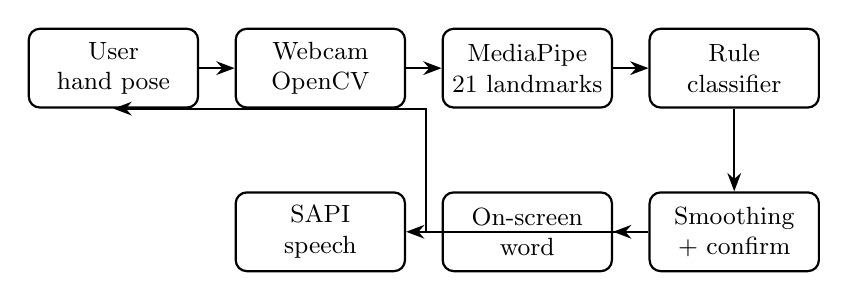
\begin{tikzpicture}[
  node distance=1.05cm and 0.45cm,
  box/.style={draw, thick, rounded corners, minimum width=2.15cm, minimum height=1.0cm, align=center, fill=white, font=\small},
  arr/.style={-Stealth, thick, black}
]
\node[box] (user) {User\\hand pose};
\node[box, right=of user] (cam) {Webcam\\OpenCV};
\node[box, right=of cam] (mp) {MediaPipe\\21 landmarks};
\node[box, right=of mp] (cls) {Rule\\classifier};
\node[box, below=of cls] (sm) {Smoothing\\+ confirm};
\node[box, left=of sm] (ui) {On-screen\\word};
\node[box, left=of ui] (tts) {SAPI\\speech};

\draw[arr] (user) -- (cam);
\draw[arr] (cam) -- (mp);
\draw[arr] (mp) -- (cls);
\draw[arr] (cls) -- (sm);
\draw[arr] (sm) -- (ui);
\draw[arr] (sm) -- (tts);
\draw[arr] (ui.west) -- ++(-0.2,0) |- (user.south);
\end{tikzpicture}

\end{adjustbox}
\caption{System architecture of GestureTalk}
\label{fig:arch}
\end{figure}

The capture layer uses OpenCV for the webcam, a horizontal flip and the display window \cite{opencv}. The perception layer uses MediaPipe Tasks HandLandmarker in VIDEO mode \cite{mediapipehl}. The classification layer applies geometry rules and named poses over a vocabulary of more than five hundred gestures. The temporal layer applies hysteresis and hold-to-confirm. The output layer draws the word on the frame and speaks it through interruptible Windows SAPI \cite{sapi}.

\section{DFD Level 0 (Context Diagram)}
\begin{figure}[H]
\centering
\begin{adjustbox}{max width=\textwidth,center}
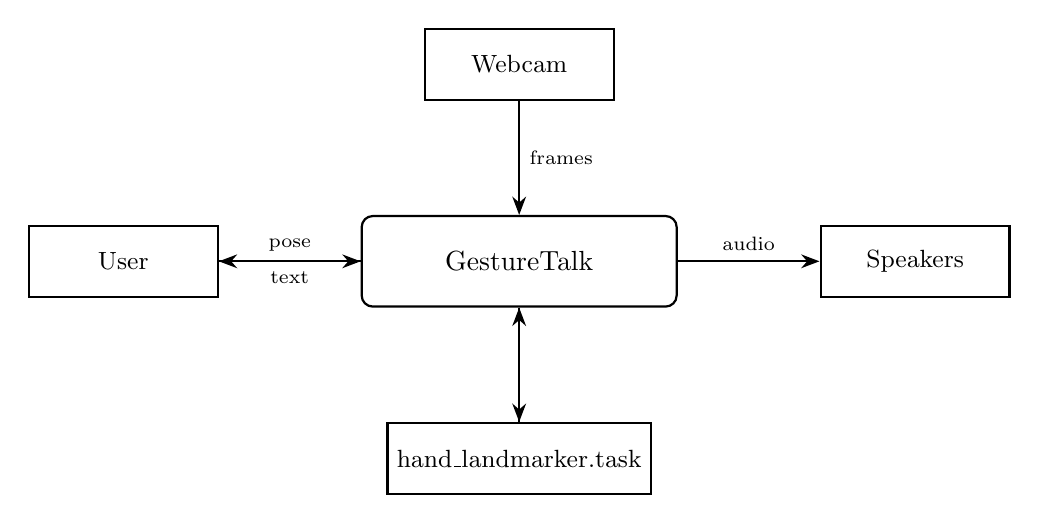
\begin{tikzpicture}[
  node distance=1.45cm and 1.8cm,
  ext/.style={draw, thick, minimum width=2.4cm, minimum height=0.9cm, fill=white, align=center, font=\small},
  proc/.style={draw, thick, rounded corners, minimum width=4.0cm, minimum height=1.15cm, fill=white, align=center},
  arr/.style={-Stealth, thick, black}
]
\node[proc] (sys) {GestureTalk};
\node[ext, left=of sys] (user) {User};
\node[ext, above=of sys] (cam) {Webcam};
\node[ext, right=of sys] (spk) {Speakers};
\node[ext, below=of sys] (model) {hand\_landmarker.task};

\draw[arr] (user) -- node[above,font=\scriptsize]{pose} (sys);
\draw[arr] (sys) -- node[below,font=\scriptsize]{text} (user);
\draw[arr] (cam) -- node[right,font=\scriptsize]{frames} (sys);
\draw[arr] (sys) -- node[above,font=\scriptsize]{audio} (spk);
\draw[arr] (sys) -- (model);
\draw[arr] (model) -- (sys);
\end{tikzpicture}

\end{adjustbox}
\caption{DFD Level 0}
\label{fig:dfd0}
\end{figure}

At the context level, GestureTalk exchanges video with the webcam, landmark inference with the on-device model file, visual feedback with the user, and audio with the speakers. Internal processing is abstracted as a single system boundary.

\section{DFD Level 1}
\begin{figure}[H]
\centering
\begin{adjustbox}{max width=\textwidth,center}
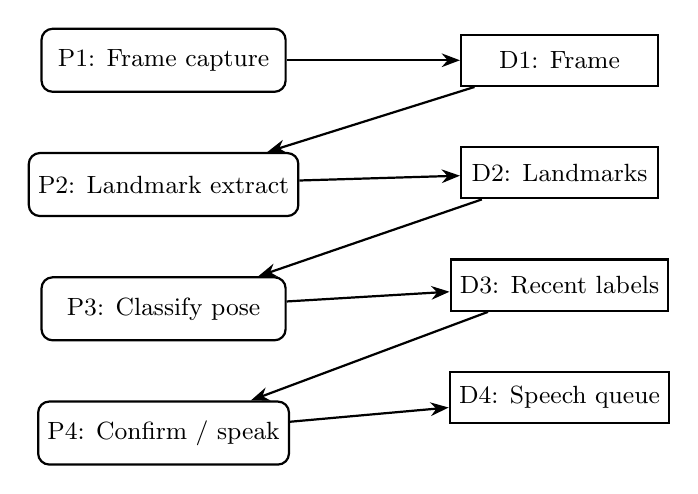
\begin{tikzpicture}[
  node distance=0.75cm and 0.95cm,
  p/.style={draw, thick, rounded corners, minimum width=3.1cm, minimum height=0.8cm, align=center, fill=white, font=\small},
  d/.style={draw, thick, minimum width=2.5cm, minimum height=0.65cm, align=center, fill=white, font=\small},
  arr/.style={-Stealth, thick, black}
]
\node[p] (p1) {P1: Frame capture};
\node[p, below=of p1] (p2) {P2: Landmark extract};
\node[p, below=of p2] (p3) {P3: Classify pose};
\node[p, below=of p3] (p4) {P4: Confirm / speak};
\node[d, right=2.2cm of p1] (d1) {D1: Frame};
\node[d, below=of d1] (d2) {D2: Landmarks};
\node[d, below=of d2] (d3) {D3: Recent labels};
\node[d, below=of d3] (d4) {D4: Speech queue};

\draw[arr] (p1) -- (d1);
\draw[arr] (d1) -- (p2);
\draw[arr] (p2) -- (d2);
\draw[arr] (d2) -- (p3);
\draw[arr] (p3) -- (d3);
\draw[arr] (d3) -- (p4);
\draw[arr] (p4) -- (d4);
\end{tikzpicture}

\end{adjustbox}
\caption{DFD Level 1}
\label{fig:dfd1}
\end{figure}

Level~1 splits the system into capture, landmark extraction, classification, confirmation, display and speech. Each process reads a small set of stores: the current frame, the landmark buffer, recent labels, the stable word and the speech queue. Shared stores make flicker control and interruption explicit.

\section{DFD Level 2 (Classification and Confirmation)}
\begin{figure}[H]
\centering
\begin{adjustbox}{max width=\textwidth,center}
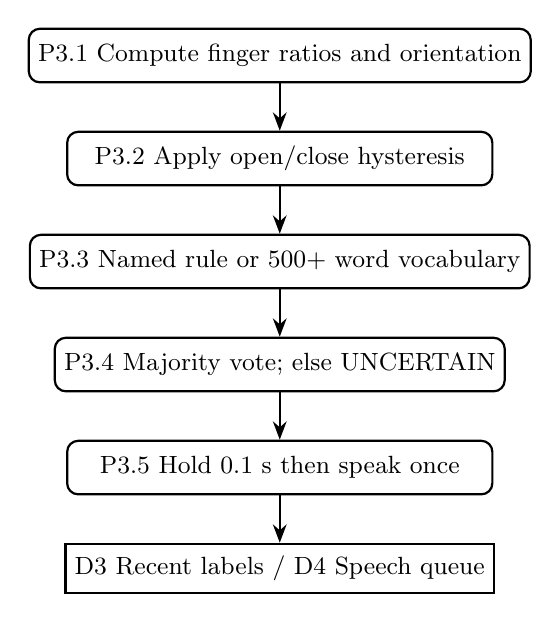
\begin{tikzpicture}[
  node distance=0.6cm,
  p/.style={draw, thick, rounded corners, minimum width=5.4cm, minimum height=0.68cm, align=center, fill=white, font=\small},
  d/.style={draw, thick, minimum width=5.4cm, minimum height=0.62cm, align=center, fill=white, font=\small},
  arr/.style={-Stealth, thick, black}
]
\node[p] (a) {P3.1 Compute finger ratios and orientation};
\node[p, below=of a] (b) {P3.2 Apply open/close hysteresis};
\node[p, below=of b] (c) {P3.3 Named rule or 500+ word vocabulary};
\node[p, below=of c] (d) {P3.4 Majority vote; else UNCERTAIN};
\node[p, below=of d] (e) {P3.5 Hold 0.1 s then speak once};
\node[d, below=of e] (s) {D3 Recent labels / D4 Speech queue};

\draw[arr] (a) -- (b);
\draw[arr] (b) -- (c);
\draw[arr] (c) -- (d);
\draw[arr] (d) -- (e);
\draw[arr] (e) -- (s);
\end{tikzpicture}

\end{adjustbox}
\caption{DFD Level 2}
\label{fig:dfd2}
\end{figure}

Level~2 expands classification into finger ratios, hysteresis, vocabulary lookup, majority vote and hold-to-confirm. Finger ratios are compared with separate open and close thresholds. Named rules such as thumbs-down NO and the OK pinch override the table. Disagreeing frames become uncertain and do not replace the last stable word.

\section{User Journey Diagram}
\begin{figure}[H]
\centering
\begin{adjustbox}{max width=\textwidth,center}
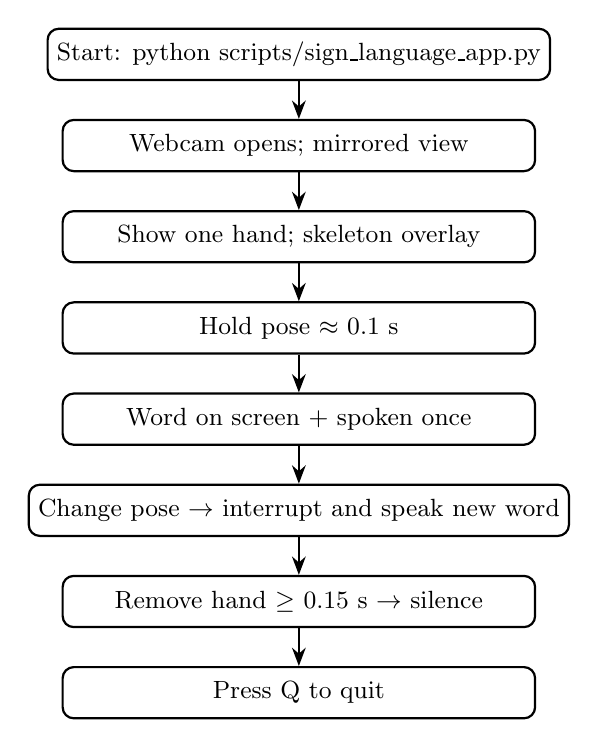
\begin{tikzpicture}[
  node distance=0.48cm,
  box/.style={draw, thick, rounded corners, minimum width=6.0cm, minimum height=0.65cm, align=center, fill=white, font=\small},
  arr/.style={-Stealth, thick, black}
]
\node[box] (a) {Start: python scripts/sign\_language\_app.py};
\node[box, below=of a] (b) {Webcam opens; mirrored view};
\node[box, below=of b] (c) {Show one hand; skeleton overlay};
\node[box, below=of c] (d) {Hold pose $\approx$ 0.1 s};
\node[box, below=of d] (e) {Word on screen + spoken once};
\node[box, below=of e] (f) {Change pose $\rightarrow$ interrupt and speak new word};
\node[box, below=of f] (g) {Remove hand $\geq$ 0.15 s $\rightarrow$ silence};
\node[box, below=of g] (h) {Press Q to quit};

\draw[arr] (a) -- (b);
\draw[arr] (b) -- (c);
\draw[arr] (c) -- (d);
\draw[arr] (d) -- (e);
\draw[arr] (e) -- (f);
\draw[arr] (f) -- (g);
\draw[arr] (g) -- (h);
\end{tikzpicture}

\end{adjustbox}
\caption{End-to-end user journey from application start to spoken word}
\label{fig:journey}
\end{figure}

The journey starts with launching \code{scripts/sign_language_app.py}. The webcam opens, the user shows one hand, holds a pose for about 0.1 seconds, sees and hears the word, may change pose, may remove the hand, and finally presses Q to quit.

\section{Entity Relationship Diagram}
There is no MySQL schema. Figure~\ref{fig:er} models runtime objects and their relationships.

\begin{figure}[H]
\centering
\begin{adjustbox}{max width=\textwidth,center}
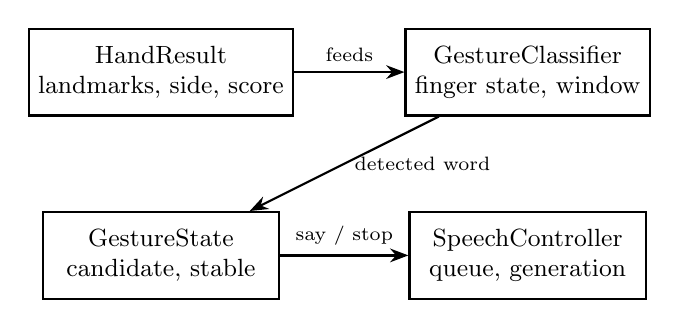
\begin{tikzpicture}[
  node distance=1.2cm and 1.4cm,
  ent/.style={draw, thick, minimum width=3.0cm, minimum height=1.1cm, align=center, fill=white, font=\small},
  arr/.style={-Stealth, thick, black}
]
\node[ent] (h) {HandResult\\landmarks, side, score};
\node[ent, right=of h] (c) {GestureClassifier\\finger state, window};
\node[ent, below=of h] (g) {GestureState\\candidate, stable};
\node[ent, below=of c] (s) {SpeechController\\queue, generation};

\draw[arr] (h) -- node[above,font=\scriptsize]{feeds} (c);
\draw[arr] (c) -- node[right,font=\scriptsize]{detected word} (g);
\draw[arr] (g) -- node[above,font=\scriptsize]{say / stop} (s);
\end{tikzpicture}

\end{adjustbox}
\caption{Runtime entity relationship diagram}
\label{fig:er}
\end{figure}

One hand result exists per detected hand, with a maximum of one hand in the current demo. The classifier owns finger hysteresis. Gesture state owns confirmation. The speech controller owns the queue and generation counter. These objects live in memory only.

\section{Use Case Diagram}
\begin{figure}[H]
\centering
\begin{adjustbox}{max width=\textwidth,center}
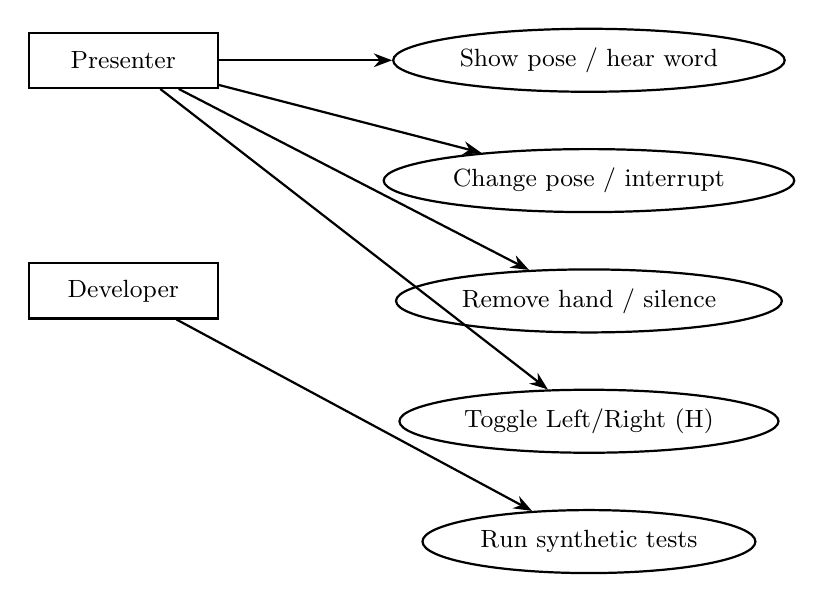
\begin{tikzpicture}[
  node distance=0.7cm and 1.2cm,
  actor/.style={draw, thick, minimum width=2.4cm, minimum height=0.7cm, fill=white, align=center, font=\small},
  use/.style={draw, thick, ellipse, minimum width=4.2cm, minimum height=0.8cm, fill=white, align=center, font=\small},
  arr/.style={-Stealth, thick, black}
]
\node[actor] (u) {Presenter};
\node[actor, below=2.2cm of u] (d) {Developer};

\node[use, right=2.2cm of u] (u1) {Show pose / hear word};
\node[use, below=of u1] (u2) {Change pose / interrupt};
\node[use, below=of u2] (u3) {Remove hand / silence};
\node[use, below=of u3] (u4) {Toggle Left/Right (H)};
\node[use, below=of u4] (u5) {Run synthetic tests};

\draw[arr] (u) -- (u1);
\draw[arr] (u) -- (u2);
\draw[arr] (u) -- (u3);
\draw[arr] (u) -- (u4);
\draw[arr] (d) -- (u5);
\end{tikzpicture}

\end{adjustbox}
\caption{Use case diagram}
\label{fig:usecase}
\end{figure}

The presenter shows a pose, changes pose, removes the hand and may toggle left and right correction. The developer runs synthetic tests.

\section{Sequence Diagram (Stable Gesture to Speech)}
\begin{figure}[H]
\centering
\begin{adjustbox}{max width=\textwidth,center}
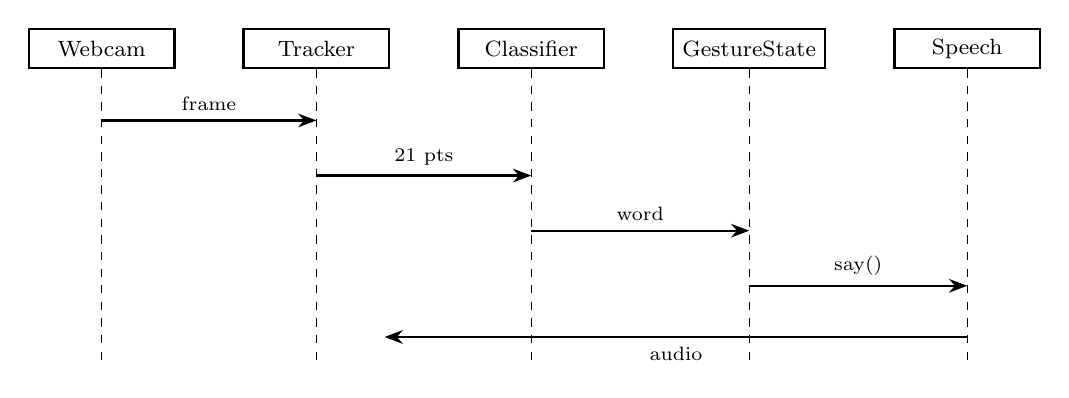
\begin{tikzpicture}[
  font=\footnotesize,
  actor/.style={draw, thick, minimum width=1.85cm, minimum height=0.5cm, align=center, fill=white},
  arr/.style={-Stealth, thick, black}
]
\node[actor] (w) {Webcam};
\node[actor, right=0.85cm of w] (t) {Tracker};
\node[actor, right=0.85cm of t] (c) {Classifier};
\node[actor, right=0.85cm of c] (g) {GestureState};
\node[actor, right=0.85cm of g] (s) {Speech};

\foreach \n in {w,t,c,g,s}
  \draw[dashed] (\n.south) -- ++(0,-3.7);

\draw[arr] ([yshift=-0.65cm]w.south) -- node[above,font=\scriptsize]{frame} ([yshift=-0.65cm]t.south);
\draw[arr] ([yshift=-1.35cm]t.south) -- node[above,font=\scriptsize]{21 pts} ([yshift=-1.35cm]c.south);
\draw[arr] ([yshift=-2.05cm]c.south) -- node[above,font=\scriptsize]{word} ([yshift=-2.05cm]g.south);
\draw[arr] ([yshift=-2.75cm]g.south) -- node[above,font=\scriptsize]{say()} ([yshift=-2.75cm]s.south);
\draw[arr] ([yshift=-3.4cm]s.south) -- node[below,font=\scriptsize]{audio} ++(-7.4,0);
\end{tikzpicture}

\end{adjustbox}
\caption{Sequence diagram for a confirmed gesture}
\label{fig:seq}
\end{figure}

The webcam loop sends a frame to the tracker, receives twenty-one points, asks the classifier for a word, waits for GestureState to confirm, and then asks the speech thread to speak. Audio returns to the user without blocking the next camera frame.

\section{Module Design}
The webcam loop, confirmation window, overlay and key handling live in \code{scripts/sign_language_app.py}. MediaPipe wrapping and skeleton drawing live in \code{src/signlang/hand_tracker.py}. Vocabulary, geometry and hysteresis live in \code{src/signlang/gestures.py}. Interruptible SAPI lives in \code{src/signlang/speech.py}. Synthetic landmark tests live in \code{tests/test_gestures.py}. The MediaPipe model file is stored at \code{models/hand_landmarker.task}.

\begin{table}[H]
\centering
\small
\caption{Source modules and responsibilities}
\label{tab:modules}
\begin{tabularx}{\textwidth}{@{}>{\raggedright\arraybackslash}p{3.6cm} L@{}}
\toprule
\textbf{Module} & \textbf{Responsibility} \\
\midrule
sign\_language\_app.py & Frame loop, confirm window, keys Q and H, overlay text \\
hand\_tracker.py & VIDEO-mode landmark detection and drawing \\
gestures.py & 500+ gesture vocabulary, named poses, handedness correction \\
speech.py & Background thread, generation counter, SAPI purge \\
test\_gestures.py & Synthetic coverage and noise protocol \\
check\_env.py & Python, packages, model, webcam and TTS checks \\
\bottomrule
\end{tabularx}
\end{table}


\chapter{Implementation}
\section{Technology Stack}
The application is written in Python 3.12 or newer. OpenCV handles capture, the selfie flip and overlay drawing \cite{opencv}. MediaPipe Tasks HandLandmarker supplies twenty-one landmarks in VIDEO mode \cite{mediapipehl,mediapipehands}. NumPy is used for distances and orientation. Speech uses Windows SAPI.SpVoice through \code{pywin32} \cite{sapi}. PyTorch, scikit-learn and torchinfo are installed for later training \cite{pytorch}. CustomTkinter is reserved for a later desktop shell. Cloud speech APIs were not used, because offline operation is a requirement.

MediaPipe 1.x does not include \code{mp.solutions.hands} in the wheel, so the Tasks API is mandatory on a current install \cite{mediapipehl}. OpenCV contrib is used because MediaPipe depends on it. Installing both \code{opencv-python} and \code{opencv-contrib-python} in the same environment causes conflicts, so only the contrib package is kept.

\section{Development Environment}
The project was developed on Windows using Visual Studio Code, a Python virtual environment and Git. Environment checks are automated by \code{scripts/check_env.py}. The MediaPipe model is downloaded by \code{scripts/download_models.py}. Synthetic tests do not require a webcam.

\section{Tracking Implementation}
\code{HandTracker} wraps HandLandmarker in VIDEO mode. Each BGR frame is converted to RGB, wrapped as a MediaPipe Image, and passed with a strictly increasing timestamp. Output is a list of hand results. Skeleton drawing uses the standard twenty-one connections. Isolating MediaPipe in one file means a future API change does not rewrite the application loop. The live window is mirrored with \code{cv2.flip(frame, 1)} so that raising the right hand appears on the right side of the screen.

\section{Classifier Implementation}
Five finger extension ratios are computed from landmark distances and compared with separate open and close thresholds. That hysteresis stops a fingertip sitting near a boundary from flipping the bit on every frame. Orientation is the wrist-to-middle-MCP vector, labelled UP, DOWN, LEFT or RIGHT. MediaPipe handedness is corrected in one place because the mirrored selfie view otherwise swaps left and right. The H key can toggle that correction during a demo.

Finger configuration, orientation and hand side index a custom vocabulary of more than five hundred everyday gestures. Words were chosen from daily life so that a short demonstration can cover greetings, family, school, food, travel, numbers, colours and common actions. Named poses used in the viva include HELLO, I LOVE YOU, YES, thumbs-down NO, PEACE, ONE POINT, FIST, ROCK ON, CALL ME, OK, THREE and FOUR. Special rules sit above the table. A closed fist with the thumb clearly below the wrist is treated as NO. An OK pose is recognised when the thumb tip meets the index tip while the other three fingers stay extended.

The classifier keeps a five-frame window. A word is emitted only if it holds at least sixty percent of that window and at least three frames have been seen. Otherwise the return value is uncertain, and the last stable overlay is left unchanged.

\section{Confirmation and Speech}
\code{GestureState} requires the candidate to remain unchanged for about 0.1 seconds. A held pose is spoken once. A different stable pose is spoken again. A stable empty or unknown state clears the last spoken word, so the same gesture can be spoken after a clear break. \code{SpeechController} starts a daemon thread, creates SAPI.SpVoice, and reads generation and word pairs from a queue. Calling \code{say()} increments the generation. Calling \code{stop()} increments it and drains the queue. The worker speaks asynchronously and purges the utterance if the generation has moved on \cite{sapi}. The camera loop never waits for speech to finish.

\section{Error Handling and Validation}
Missing webcam frames print a message and break the loop. A missing model file raises a clear error that tells the user to run the download script. Speech exceptions are logged without stopping the camera. Landmark aspect-ratio correction multiplies $x$ by frame width over height so stretched cameras do not distort distances. If no hand is present, the classifier is reset so stale finger state does not leak into the next detection.

\section{Limitations}
The classifier is a project-specific vocabulary. It is not American Sign Language or Indian Sign Language. Lighting, camera angle and two-handed signs are outside the current model. There is no held-out human dataset and no confusion matrix yet. Those limits are accepted for this stage of Project-II. They are not hidden behind a claim of language-level accuracy.

\section{Technology Stack Summary}
\begin{table}[H]
\centering
\small
\caption{Technology stack}
\label{tab:stack}
\begin{tabularx}{\textwidth}{@{}>{\raggedright\arraybackslash}p{3.2cm} >{\raggedright\arraybackslash}p{2.6cm} L@{}}
\toprule
\textbf{Technology} & \textbf{Category} & \textbf{Role} \\
\midrule
Python 3.12+ & Language & Application, tests and geometry \\
OpenCV \cite{opencv} & Vision & Capture, flip, overlay and window \\
MediaPipe Tasks \cite{mediapipehl} & Perception & 21 landmarks in VIDEO mode \\
NumPy & Numerics & Distances, orientation and noise tests \\
Windows SAPI \cite{sapi} & Speech & Offline, interruptible TTS \\
PyTorch \cite{pytorch} & Planned ML & Later MLP training \\
scikit-learn & Planned ML & Metrics and person-wise split \\
CustomTkinter & Planned UI & Later desktop shell \\
\bottomrule
\end{tabularx}
\end{table}


\chapter{Results and Screenshots}
\section{Demonstration Setup}
The screenshots in this chapter were taken from the live Windows application running on the development laptop. The default webcam was used. The user sat at a desk, faced the camera, and held one hand inside the frame. Lighting was ordinary indoor room light. No cloud service was used during the demonstration.

\section{Hand Detection}
Figure~\ref{fig:hand} shows the tracker overlay. The skeleton follows the twenty-one MediaPipe landmarks, and the window remains a mirrored selfie view. This is the first check in a viva: if the skeleton does not sit on the hand, later classification cannot be trusted.

\begin{figure}[H]
\centering
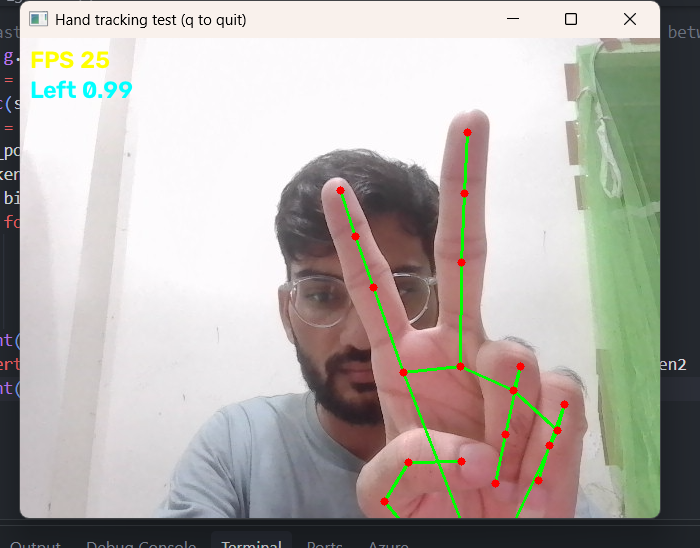
\includegraphics[width=0.72\textwidth]{Hand_detection.png}
\caption{Live hand detection with MediaPipe landmark overlay}
\label{fig:hand}
\end{figure}

\section{Gesture to Text}
Figure~\ref{fig:sign} shows a recognised pose converted into on-screen text. After the hand is held steady, the overlay stops saying ``Checking...'' and shows the confirmed word. The same word is queued for speech. Diagnostic text on the window reports the corrected hand side, the finger bit pattern and the pointing orientation. Those fields are useful while explaining the classifier in a viva, because they show why a particular table entry was chosen.

\begin{figure}[H]
\centering
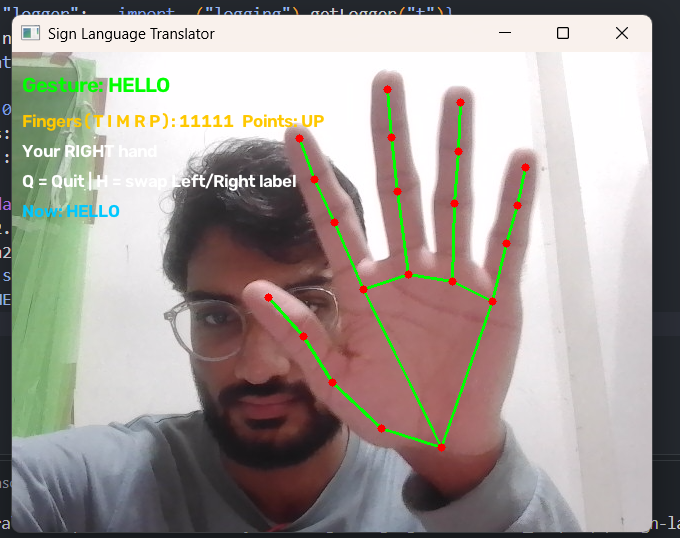
\includegraphics[width=0.72\textwidth]{sign_language.png}
\caption{Recognised gesture shown as text on the live window}
\label{fig:sign}
\end{figure}

\section{No Hand State}
Figure~\ref{fig:nohand} shows the empty-frame behaviour. When the hand leaves the camera, the overlay returns to ``No hand detected''. After about 0.15 seconds the speech controller stops the current utterance and drops pending words. This is an important result for a live demo. Without it, the last spoken word would keep playing after the user has already put the hand down.

\begin{figure}[H]
\centering
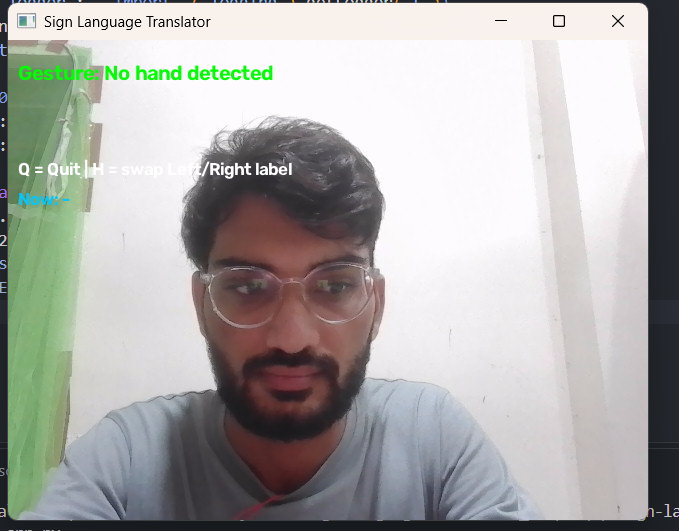
\includegraphics[width=0.72\textwidth]{when_no_hand.png}
\caption{Application state when no hand is visible}
\label{fig:nohand}
\end{figure}

\section{Large Vocabulary}
Figure~\ref{fig:more} shows that the system is not limited to a handful of named signs. More than five hundred everyday gestures were added for this project. The extra words cover greetings, family, school, food, travel, numbers, colours and common actions. In the demonstration, changing from one stable pose to another updates the overlay and interrupts the previous speech so the new word is heard without waiting.

\begin{figure}[H]
\centering
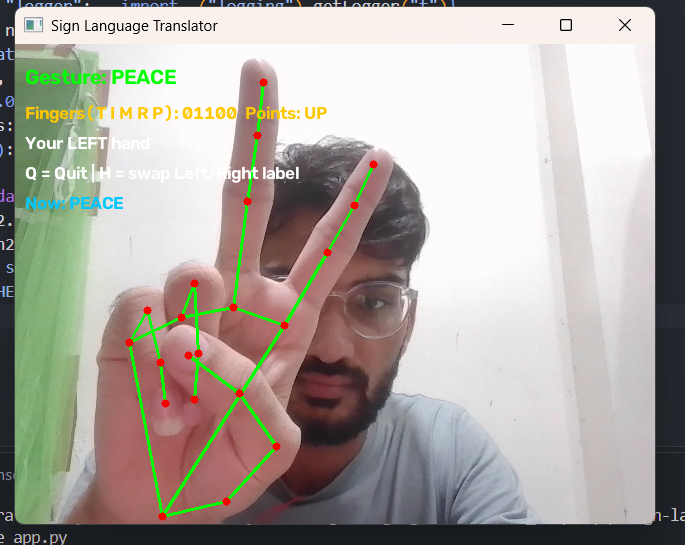
\includegraphics[width=0.72\textwidth]{more_gestures.png}
\caption{Live recognition from the 500+ gesture vocabulary}
\label{fig:more}
\end{figure}

\section{Synthetic Tests}
Webcam-free tests in \code{tests/test_gestures.py} build synthetic landmarks for finger patterns and orientations. Named poses such as HELLO, I LOVE YOU, YES, PEACE and FIST return the expected labels. Thumbs-down is recognised as NO. Left and right hands produce different table entries for the same finger pattern after handedness correction. Aspect-ratio correction is checked so that a stretched frame does not change the label. A short hold-to-confirm sequence is also simulated by feeding GestureState at thirty updates per second.

Under a synthetic noise protocol, filtered YES and HELLO labels remained above ninety percent, and a five-pose burst was spoken in the expected order. These numbers describe the synthetic protocol, not a human sign-language benchmark. They are reported here because they document anti-flicker behaviour without claiming ASL or ISL accuracy.

\section{Observed Runtime Behaviour}
On the development laptop the camera loop stayed interactive while speech was playing. Changing pose while a word was still being spoken cut off the old audio. Holding the same pose did not repeat the word. Removing the hand silenced the speakers. Those observations match the design of the generation counter in \code{SpeechController}. Frame rate was not formally benchmarked against ONNX in this stage. Qualitatively, tracking and overlay remained usable for a live viva on CPU.


\chapter{Conclusion and Future Scope}
\section{Conclusion}
This report presented GestureTalk, a real-time sign language recognition, text conversion and speech generation system built as a Project-II prototype. The application reads one hand from a laptop webcam, classifies a custom vocabulary of more than five hundred gestures, shows the recognised English word on the screen, and speaks that word through the Windows speech engine without using the internet.

The engineering work of this stage sits in the complete local pipeline rather than in a published accuracy number. MediaPipe Tasks supplies current landmark tracking. Geometry rules and named poses convert landmarks into words. Hysteresis, majority vote and a short confirmation window keep the overlay steady. A background speech thread lets a new pose interrupt the previous sentence. Synthetic tests cover named poses, handedness correction and noisy landmarks without a camera.

The system is a working demonstration, not a full interpreter of American Sign Language or Indian Sign Language. That limit is part of the conclusion, not an afterthought. Within the chosen scope, the project shows that a student implementation can go from camera to spoken word in real time, with a large everyday vocabulary, on an ordinary Windows laptop.

\section{Future Scope}
The next natural step is to collect landmark sequences from several people and train a small multilayer perceptron, keeping a person-wise split so that evaluation does not leak the same signer into both sides. A CustomTkinter shell can then wrap the OpenCV window, a history of recognised words, and simple controls for volume and handedness. ONNX export would allow a fair FPS and latency table on CPU. Two-handed poses, motion signs and a small phrase buffer are later extensions. Those items belong to later work. They are not claimed as results of the present prototype.


\nocite{*}
\bibliography{report}
\bibliographystyle{unsrt}

\end{document}
